\documentclass[12pt]{article}
\usepackage[english]{babel}
\usepackage{natbib}
\usepackage{url}
\usepackage[utf8x]{inputenc}
\usepackage{amsmath}
\usepackage{graphicx}
\graphicspath{{images/}}
\usepackage{parskip}
\usepackage{fancyhdr}
\usepackage{vmargin}
\usepackage{float}
\usepackage[utf8]{vietnam}
\setmarginsrb{3 cm}{2.5 cm}{3 cm}{2.5 cm}{1 cm}{1.5 cm}{1 cm}{1.5 cm}

\title{E-Learning System for Faculty of Computer Science and Engineering}                             % Title
\author{
  Nguyen Minh Tri\\
  Pham Duc Minh Chau\\
  Le Huynh Duy Thai\\
 }
\date{\today}                                           % Date

\makeatletter
\let\thetitle\@title
\let\theauthor\@author
\let\thedate\@date
\makeatother

\pagestyle{fancy}
\fancyhf{}
\lhead{\thetitle}
\cfoot{\thepage}

\begin{document}
%%%%%%%%%%%%%%%%%%%%%%%%%%%%%%%%%%%%%%%%%%%%%%%%%%%%%%%%%%%%%%%%%%%%%%%%%%%%%%%%%%%%%%%%%

\begin{titlepage}
    \centering
    \vspace*{0.5 cm}
    
\includegraphics[scale = 0.5]{hcmut.png}\\[1.0 cm]   % University Logo
    \textsc{\Large Ho Chi Minh City University of Technology}\\[1.0 cm]   % University Name
    \textsc{\Large Advanced Programming}\\[0.5 cm]               % Course Code
    \textsc{\large Assignment 1}\\[0.5 cm]               % Course Name
    \rule{\linewidth}{0.2 mm} \\[0.4 cm]
    { \LARGE \bfseries \thetitle}\\
    \rule{\linewidth}{0.2 mm} \\[1.5 cm]
    
    \begin{minipage}{0.4\textwidth}
        \begin{flushleft} \large
            \emph{Member:}\\
            \theauthor
            \end{flushleft}
            \end{minipage}~
            \begin{minipage}{0.4\textwidth}
            \begin{flushright} \large
            \emph{Student ID:} \\
            1770026 \\
            1770316\\
            1770320\\                                  % Your Student Number
        \end{flushright}
    \end{minipage}\\[2 cm]
    
    {\large \thedate}\\[2 cm]
 
    \vfill
    
\end{titlepage}

%%%%%%%%%%%%%%%%%%%%%%%%%%%%%%%%%%%%%%%%%%%%%%%%%%%%%%%%%%%%%%%%%%%%%%%%%%%%%%%%%%%%%%%%%

\renewcommand{\contentsname}{Mục Lục}
\tableofcontents
\pagebreak

%%%%%%%%%%%%%%%%%%%%%%%%%%%%%%%%%%%%%%%%%%%%%%%%%%%%%%%%%%%%%%%%%%%%%%%%%%%%%%%%%%%%%%%%%

\section{Mục Tiêu}
Phát triển một ứng dụng hỗ trợ học tập online. Nhằm đáp ứng nhu cầu cho hai đối tượng là sinh viên và giảng viên bao gồm các chức năng cơ bản như sau:
\begin{itemize}
\item Sinh viên:
 \begin{itemize}
 \item Bảng thông báo lớn: chứa tất cả các thông báo từ các khóa học mà sinh đó đang tham gia.
 \item Bảng thông báo của môn học: chứa các thông báo của khóa học mà sinh viên đang chọn.
 \item Assignment: Cho phép sinh viên đang tham gia khóa học xem các assignment của khóa học đó, cũng như là nộp bài cho assignmet đó, cho phép sinh viên nộp nhiều lần. Hỗ trợ đính kèm nhiều file.
 \item Thảo luận: có chức năng như 1 forum nhỏ để sinh viên có thể thảo luận ý kiến với giảng viên cũng như là các sinh viên khác.
 \item Sổ điểm: Cho phép sinh viên xem điểm của mình.
 \item Tài nguyên môn học: Là nơi sinh viên sẽ tải các tài nguyên của môn học như là slides, tài liệu tham khảo…
 \end{itemize}
\item Giảng viên:
 \begin{itemize}
 \item Thông báo: có quyền thêm xóa sửa thông báo cho môn học mà mình đang phụ trách.
 \item Assignment: Giảng viên có thể thêm một assignment mới, đính kèm nhiều file. Có thể sửa xóa những assignment đã đăng. Xem được danh sách nộp bài của sinh viên.
 \item Thảo luận: cũng có chức năng tương tự với sinh viên, có thể trả lời các bạn sinh viên hỏi.
 \item Bảng điểm: Cho phép giảng viên nhập điểm. Ví dụ như 15 phút, Lab, tuts, điểm thi,…. Hỗ trợ nhập thông qua file Excel. Xóa các điểm đã nhập.
 \item Tài nguyên: Giảng viên sẽ thêm file, xóa file liên quan đến khóa học.
 \end{itemize}
\end{itemize}

\newpage

\section{Thiết kế}
\begin{itemize}
\item Thiết kế tổng thể
\begin{figure}[H]
\centering
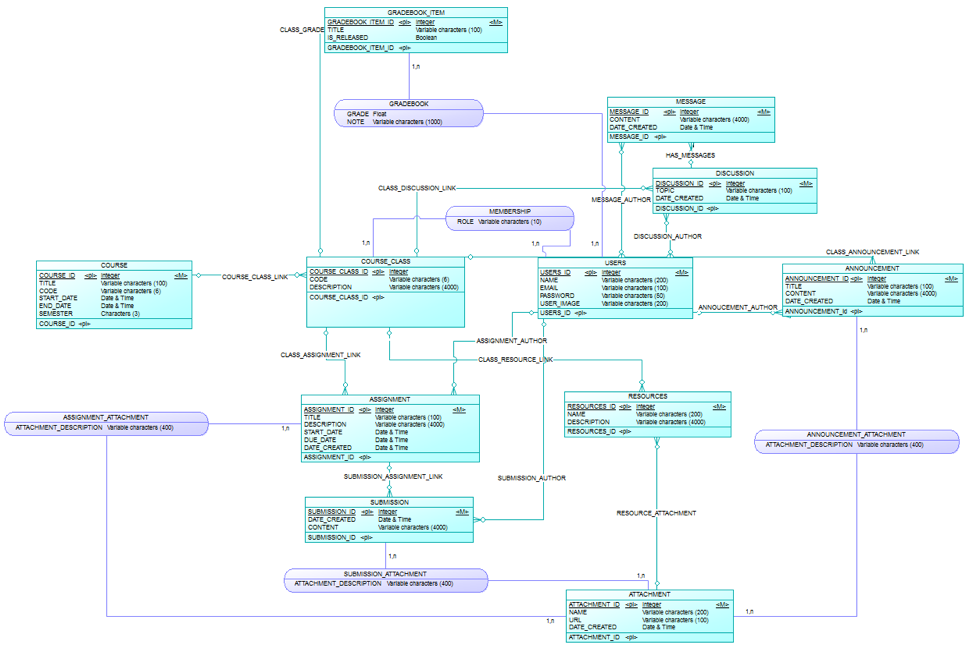
\includegraphics[scale = 0.9]{general.png}
\caption{Thiết Kế Tổng Thể}
\end{figure}

\item Thiết kế hệ thống thông báo
\begin{figure}[H]
\centering
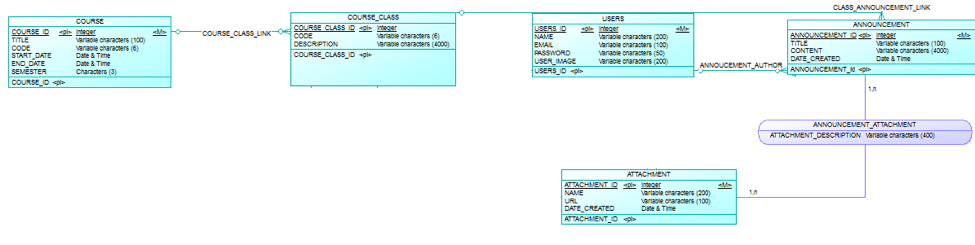
\includegraphics[scale = 0.9]{noti.png}
\caption{Hệ Thống Thông Báo}
\end{figure}

\newpage

\item Thiết kế hệ thống thảo luận
\begin{figure}[H]
\centering
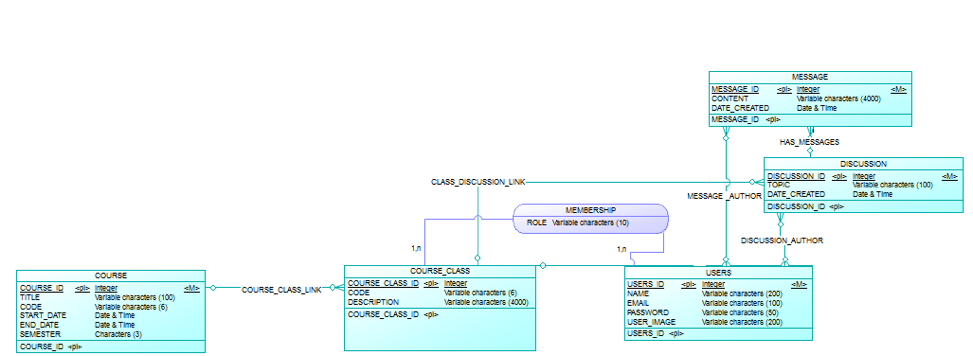
\includegraphics[scale = 0.9]{discuss.png}
\caption{Hệ Thống Thảo Luận}
\end{figure}

\item Thiết kế hệ thống điểm số
\begin{figure}[H]
\centering
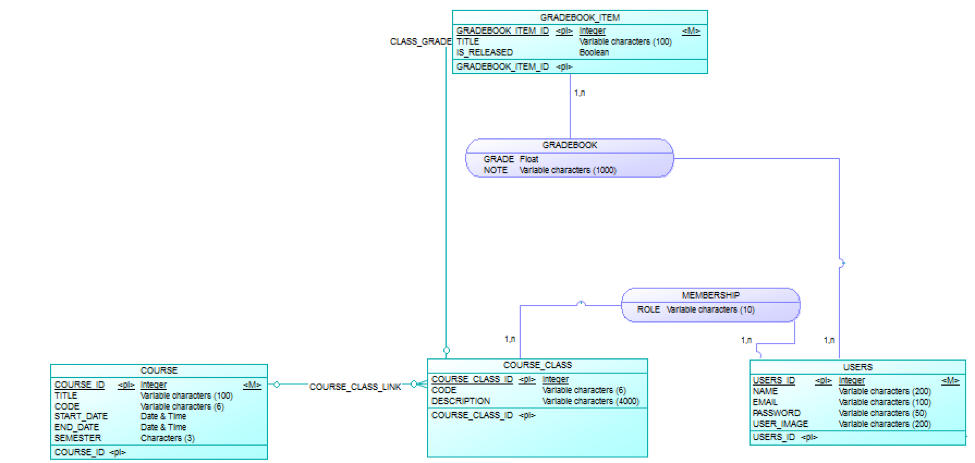
\includegraphics[scale = 0.9]{score.png}
\caption{Hệ Thống Điểm Số}
\end{figure}

\newpage

\item Thiết kế hệ thống tài nguyên
\begin{figure}[H]
\centering
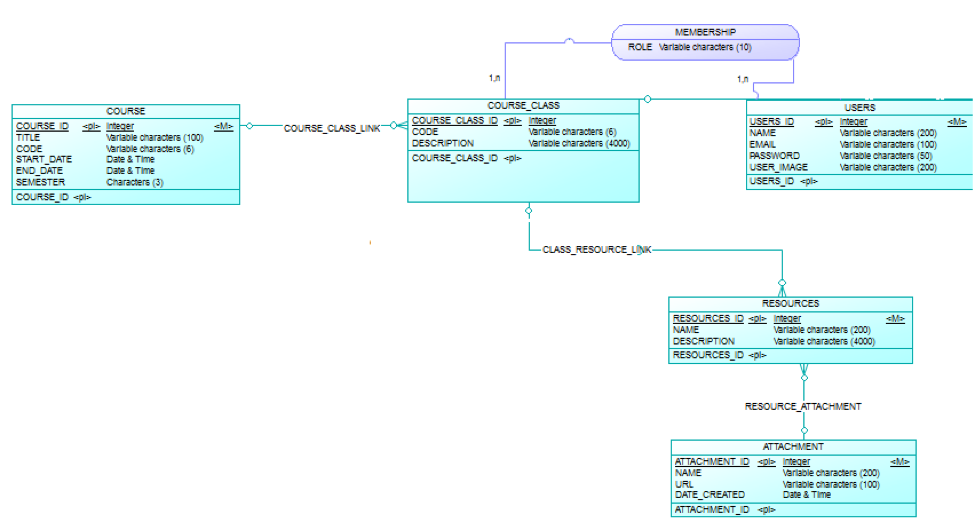
\includegraphics[scale = 0.9]{resource.png}
\caption{Hệ Thống Tài Nguyên}
\end{figure}

\item Thiết kế hệ thống bài tập lớn
\begin{figure}[H]
\centering
\includegraphics[scale = 0.9]{Assignment.png}
\caption{Hệ Thống Bài Tập Lớn}
\end{figure}

\end{itemize}


\section{Giải pháp công nghệ}
Sử dụng Power Design để thiết kế về mặt ý niệm. Vì công cụ hỗ trợ sinh ra code xây dựng cơ sở dữ liệu nên quyết định sử dụng SQL Server cho phần database.\\
Về phần máy chủ, nhóm quyết định sử dụng Nodejs và Expressjs để phát triển dưới dạng web service giao tiếp với ứng dụng web Angular thông qua JSON. Vì xây dựng dưới dạng web service nên ứng dụng có thể mở rộng ra trên di động.

\begin{figure}[H]
\centering
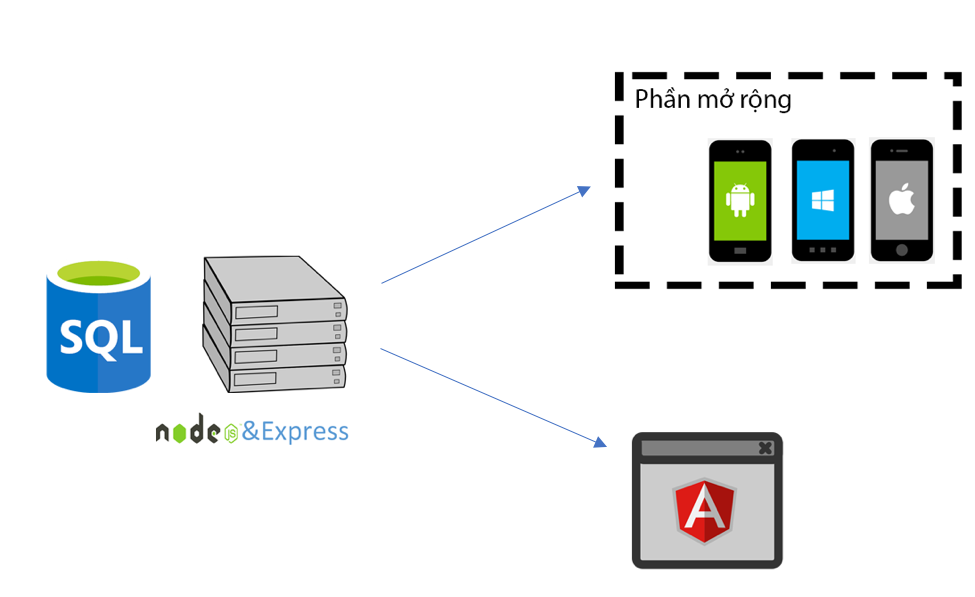
\includegraphics[scale = 0.9]{tech.png}
\caption{Giải Pháp Công Nghệ}
\end{figure}

\subsection{Angular Js}
\begin{itemize}
\item Angular là một bộ Javascript Framework rất mạnh và thường được sử dụng để xây dựng project Single Page Application (SPA). Nó hoạt động dựa trên các thuộc tính mở rộng HTML (các thuộc tính theo quy tắc của Angular). Đây là một Framework mã nguồn mở hoàn toàn miễn phí và được hàng ngàn các lập trình viên trên thế giới ưa chuộng và sử dụng. Framework này được thế hệ Web 2.0 phát triển khá mạnh ở nước ngoài, tuy nhiên ở Việt Nam thì vẫn chưa thông dụng lắm.
\item Dữ liệu hai chiều  là tính năng đáng chú ý nhất của AngularJS, chủ yếu là làm giảm sự phụ thuộc vào máy chủ khi giao diện có sự thay đổi. Thay vào đó, các mẫu (templates) được hiển thị bằng HTML thuần, theo dữ liệu chứa trong “\$scope” được định nghĩa thông qua các “model”. “\$scope” trong AngularJS sẽ phát hiện ra các thay đổi của các biến trong “script” sau đó tiến hành cập nhật các phần tử trong HTML thông qua các “controller”. Tương tự như vậy, bất kỳ sự thay đổi nào từ các “model” trong HTML cũng sẽ làm thay đổi các biến trong “script” dưới “\$scope”. Điều này giúp tăng tốc việc hiển thị dữ liệu thay vì phải tải lại trang web hoặc dễ dàng hơn là sử dụng DOM.
\item	Các đặc tính của Angular Js:
 \begin{itemize}
 \item AngularJS là một Framwork phát triển dựa trên Javascript để tạo các ứng dụng web phong phú.
 \item AngularJS thường dùng để phát triển frontend (giao diện khách hàng) thông qua các API để gọi data, sử dụng mô hình MVC rất mạnh mẽ.
 \item Mã nguồn AngularJS tự động điều chỉnh để phù hợp với các trình duyệt khác nhau nên không cần phải lo vấn đề tương thích trình duyệt.
 \item Angular là mã nguồn mở, hoàn toàn miễn phí và được phát triển bởi hàng ngàn các lập trình viên trên thế giới.
 \item Nhìn chung có thể hiểu khi làm việc với AngularJS giống như là đang làm việc với Ajax, sử dụng cớ chế bind data, hoạt động theo mô hình MVC và sử dụng service để tương tác với dữ liệu từ server. Để rõ hơn thì chúng ta tìm hiểu các tính năng cố lõi của nó.
 \end{itemize}
\item Các tính năng cốt lõi của AngularJs:
\begin{itemize}
 \item Data-binding: (liên kết dữ liệu) tự động đồng bộ dữ liệu giữa model và view.
 \item Scope: (Phạm vi) Đây là những đối tượng kết nối giữa Controller và View.
 \item Controller: Đây là những hàm javascript xử lý kết hợp với bộ điều khiển Scope.
 \item Service: Như đã đề cập ở trên, AngularJS sử dụng các API được xây dựng từ các web service (PHP, ASP) để thao tác với cơ sở dữ liệu.
 \item Filters: Bộ lọc lọc ra các thành phẩn của một mảng và trả về mảng mới.
 \item Directives:  đánh dấu vào các yếu tố của DOM, nghĩa là sẽ tạo ra các thẻ HTML tùy chỉnh.
 \item Templates: hiển thị thông tin từ controller, đây là một thành phần của views.
 \item Routing:  chuyển đổi giữa các action trong controller.
 \item MVC: Mô hình chia thành phần riêng biệt thành Model, View, Controller. Đây là một mô hình khá hay nhưng trong Angular thì nó được chế biến lại một chút gần giốn với MVVM (Model View View Model).
 \item Deep Linking: Liên kết sâu, cho phép bạn mã hóa trạng thái của ứng dụng  trong các URL  để nó có thể đánh dấu được với công cụ tìm kiếm.
 \item Dependency Injection: Angular giúp các nhà phát triển tạo ứng dụng  dễ dàng hơn để phát triển, hiểu và thử nghiệm dễ dàng.
 \item Sau đây là hình ảnh mô hình các thành phần quan trọng trong AngularJS:
\begin{figure}[H]
\centering
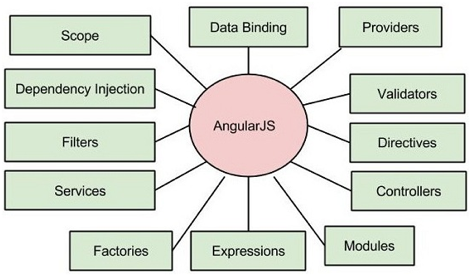
\includegraphics[scale = 1]{angular.png}
\caption{Các Thành Phần của Angular Js}
\end{figure}
\end{itemize}
\item	Ưu điểm của AngularJs:
\begin{itemize}
 \item Angular cho phép tạo ra các ứng dụng một cách đơn giản, code sạch.
 \item Angular sử dụng data bind giống .NET với tính năng liên kết với HTML nên giúp người dùng cảm thấy dễ chịu.
 \item Angular có thể chạy trên hầu hết các trình duyệt điện thoại thông minh.
\end{itemize}
\item Nhược điểm của Angular Js:
\begin{itemize}
\item Không an toàn: Được phát triển từ javascript nên nó không an toàn, phía máy chủ phải thường xuyên xác nhận quyền để hệ thống chạy trơn tru.
\item Phụ thuộc: Nếu người dùng vô hiệu hóa javascript thì coi như không thể chạy được.
\end{itemize}
\end{itemize}

\subsection{Node Js}
\begin{itemize}
\item	Giới thiệu
\begin{itemize}
 \item Node.js là một nền tảng chạy trên môi trường V8 JavaScript runtime - một trình thông dịch JavaScript cực nhanh chạy trên trình duyệt Chrome. Bình thường thì bạn cũng có thể tải bộ V8 và nhúng nó vào bất cứ thứ gì; Node.js làm điều đó đối với các web server. JavaScript suy cho cùng cũng chỉ là một ngôn ngữ - vậy thì không có lý do gì để nói nó không thể sử dụng trên môi trường server tốt như là trong trình duyệt của người dùng được.
 \item Trong một môi trường server điển hình LAMP (Linux-Apache-MySQL-PHP), chúng ta có một web server là Apache hoặc NGINX nằm dưới, cùng với PHP chạy trên nó. Mỗi một kết nối tới server sẽ sinh ra một thread mới, và điều này khiến ứng dụng nhanh chóng trở nên chậm chạp hoặc quá tải - cách duy nhất để hỗ trợ nhiều người dùng hơn là bằng cách bổ sung thêm nhiều máy chủ. Đơn giản là nó không có khả năng mở rộng tốt. Nhưng với Node.js thì điều này không phải là vấn đề. Không có một máy chủ Apache lắng nghe các kết nối tới và trả về mã trạng thái HTTP – người dùng sẽ phải tự quản lý kiến trúc lõi của máy chủ đó. May mắn thay, có một số module giúp thực hiện điều này được dễ dàng hơn, nhưng công việc này vẫn gây cho người quản lý một chút khó khăn khi mới bắt đầu. Tuy nhiên, kết quả thu được là một ứng dụng web có tốc độ thực thi cao.
 \item JavaScript là một ngôn ngữ dựa trên sự kiện, vì vậy bất cứ thứ gì xảy ra trên server đều tạo ra một sự kiện non-blocking. Mỗi kết nối mới sinh ra một sự kiện; dữ liệu nhận được từ một upload form sinh ra một sự kiện data-received; việc truy vấn dữ liệu từ database cũng sinh ra một sự kiện. Trong thực tế, điều này có nghĩa là một trang web Node.js sẽ chẳng bao giờ bị khóa (lock up) và có thể hỗ trợ cho hàng chục nghìn user truy cập cùng lúc. Node.js đóng vai trò của server - Apache - và thông dịch mã ứng dụng chạy trên nó. Giống như Apache, có rất nhiều module (thư viện) có thể được cài đặt để bổ sung thêm các đặc trưng và chức năng - như lưu trữ dữ liệu, hỗ trợ file Zip, đăng nhập bằng Facebook, hoặc các cổng thanh toán. Dĩ nhiên, nó không có nhiều thư viện như PHP, nhưng Node.js vẫn đang ở trong giai đoạn ban đầu và có một cộng đồng rất mạnh mẽ ở đằng sau nó.
 \item Một khái niệm cốt lõi của Node.js đó là các function bất đồng bộ (asynchronous functions) - vì vậy về cơ bản thì mọi thứ chạy trên nền tảng này. Với hầu hết các ngôn ngữ kịch bản máy chủ, chương trình phải đợi mỗi function thực thi xong trước khi có thể tiếp tục chạy tiếp. Với Node.js, cần xác định các function sẽ chạy để hoàn thành một tác vụ nào đó, trong khi phần còn lại của ứng dụng vẫn chạy đồng thời. Nó là một chủ đề phức tạp mà tôi sẽ không đi vào quá sâu trong bài viết này, nhưng đó là một trong những đặc trưng tiêu biểu của Node.js, vì vậy việc nắm vững nó là điều hết sức quan trọng.
\end{itemize}
\item Ưu điểm
\begin{itemize}
 \item Đầu tiên là ưu điểm về tốc độ thực thi và khả năng mở rộng. Node.js có tốc độ rất nhanh. Đó là một yêu cầu khá quan trọng khi là một startup đang cố gắng tạo ra một sản phẩm lớn và muốn đảm bảo có thể mở rộng nhanh chóng, đáp ứng được một lượng lớn người dùng khi trang web của phát triển lên. 
 \item Node.js có thể xử lý hàng ngàn kết nối đồng thời trong khi PHP sẽ bị sụp đổ.Các lợi ích về tốc độ thực thi và khả năng mở rộng là khá cao.
\end{itemize}
\item Nhược  điểm
\begin{itemize}
 \item Giống như hầu hết các công nghệ mới, việc triển khai Node.js trên host không phải là điều dễ dàng. Nếu bạn có một web hosting xài chung, chúng ta không thể đơn giản tải lên một ứng dụng Node.js và mong chờ nó hoạt động tốt. VPS và dedicated server là một sự lựa chọn tốt hơn - chúng ta có thể cài đặt Node.js trên chúng. Thậm chí dễ hơn là sử dụng một dịch vụ có khả năng mở rộng như là Heroku, và chúng ta có thể hoàn toàn an tâm để phát triển trang web của mình trên đó - chúng ta chỉ cần trả tiền khi cần thêm nhiều tài nguyên hơn.
\end{itemize}
\end{itemize}
\subsection{Express JS}
\begin{itemize}
\item Là một framework nhỏ, linh hoạt, được thiết kế cho việc xây dựng ứng dụng web đơn trang, nhiều trang và hỗn hợp ứng dụng web node.js. 
\item Framework giúp cho việc phát triển ứng dụng được rút ngắn đi rất nhiều. Cũng như các framework dựa trên những ngôn ngữ khác như Rails (Ruby); Django (Python); Laravel, CakePHP (PHP)... Express được xây dựng dựa trên Node.js. Vậy nó có ưu điểm gì để ta lựa chọn cho việc phát triển ứng dụng.
\item Express hỗ trợ việc phát triển ứng dụng theo mô hình MVC, mô hình phổ biến cho việc lập trình web hiện nay.
\item Cho phép định nghĩa Middleware hỗ trợ cho việc tổ chức và tái sử dụng code.
\item Hỗ trợ REST API.
\end{itemize}
\newpage

\section{Kết quả hiện thực}

\begin{figure}[H]
\centering
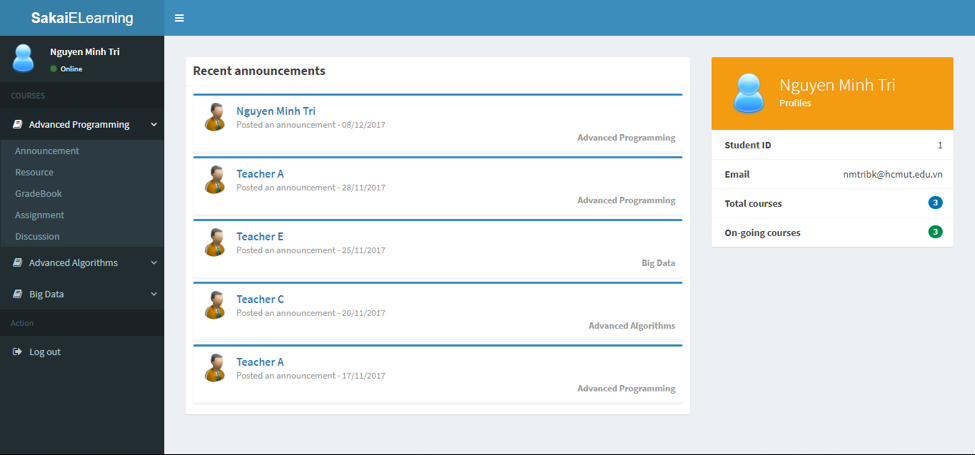
\includegraphics[scale = 1]{sakai1.png}
\caption{Trang chủ sau khi Login}
\end{figure}

\begin{figure}[H]
\centering
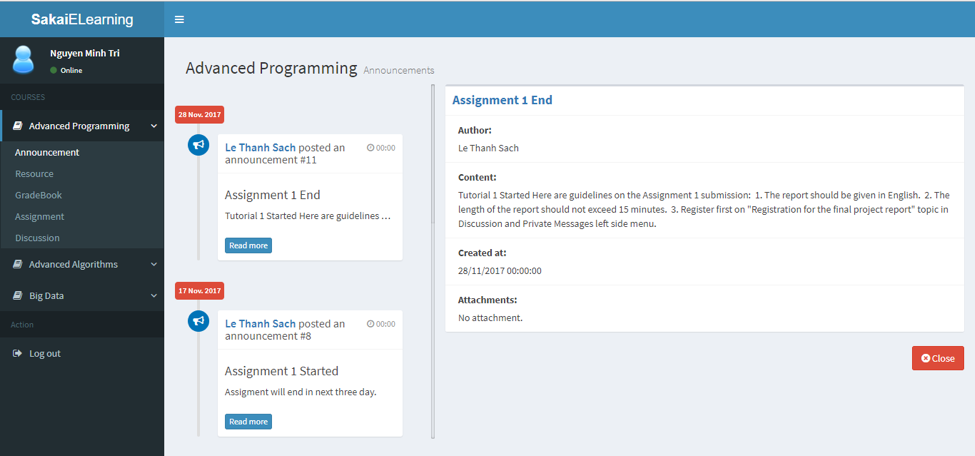
\includegraphics[scale = 1]{sakai2.png}
\caption{Trang thông báo của từng môn }
\end{figure}

\begin{figure}[H]
\centering
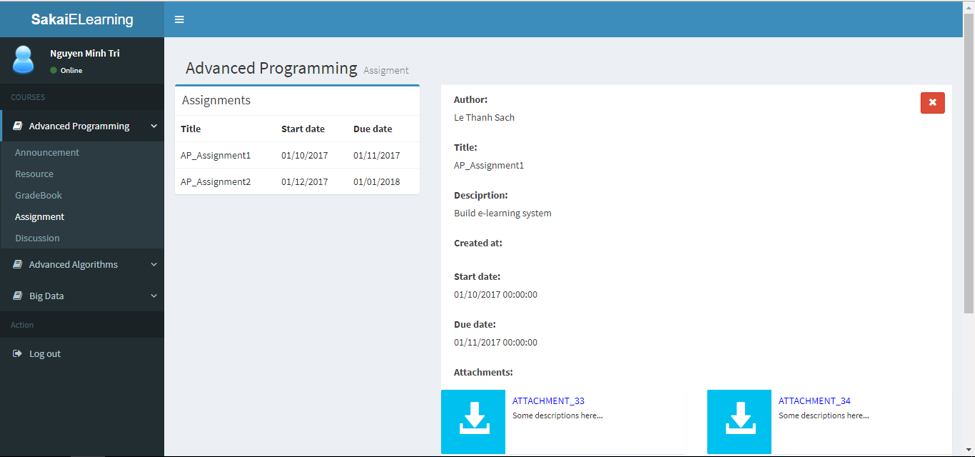
\includegraphics[scale = 1]{sakai3.png}
\caption{Trang thông tin về các Assignment trong từng môn học}
\end{figure}

\begin{figure}[H]
\centering
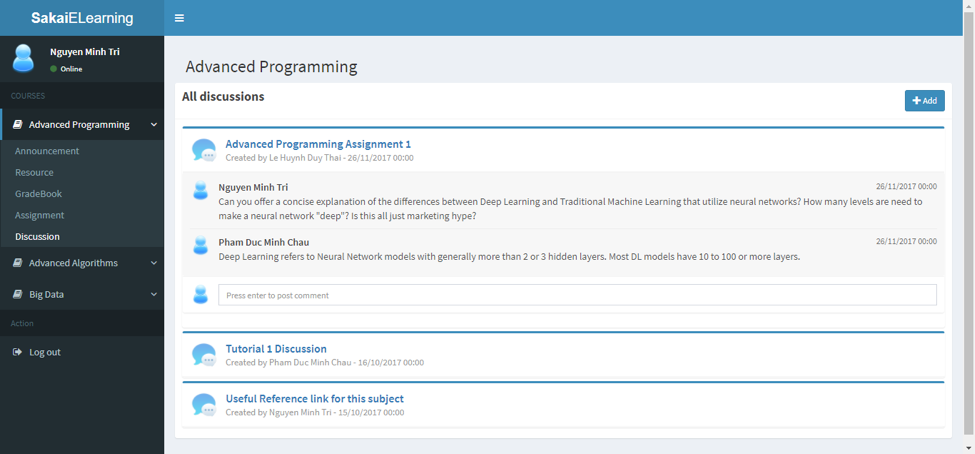
\includegraphics[scale = 1]{sakai4.png}
\caption{Trang thảo luận giữa các sinh viên và giáo viên}
\end{figure}

\begin{figure}[H]
\centering
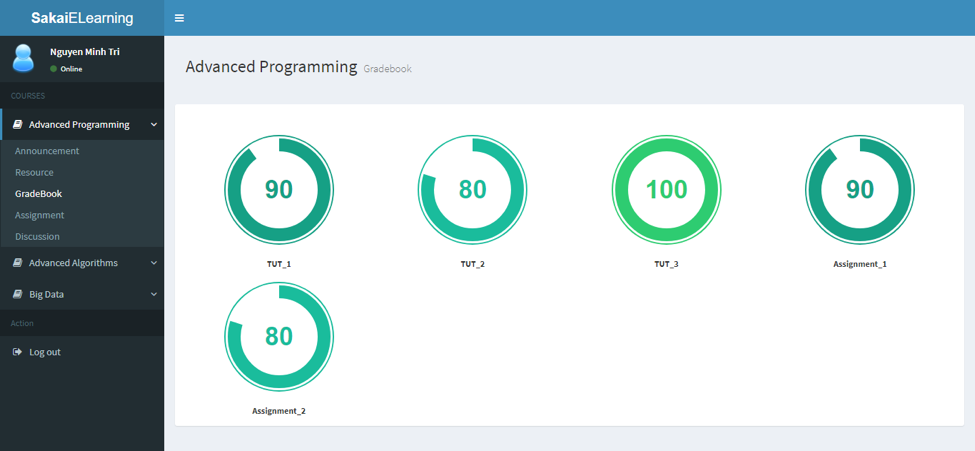
\includegraphics[scale = 1]{sakai5.png}
\caption{Trang xem điểm của từng môn }
\end{figure}

\begin{figure}[H]
\centering
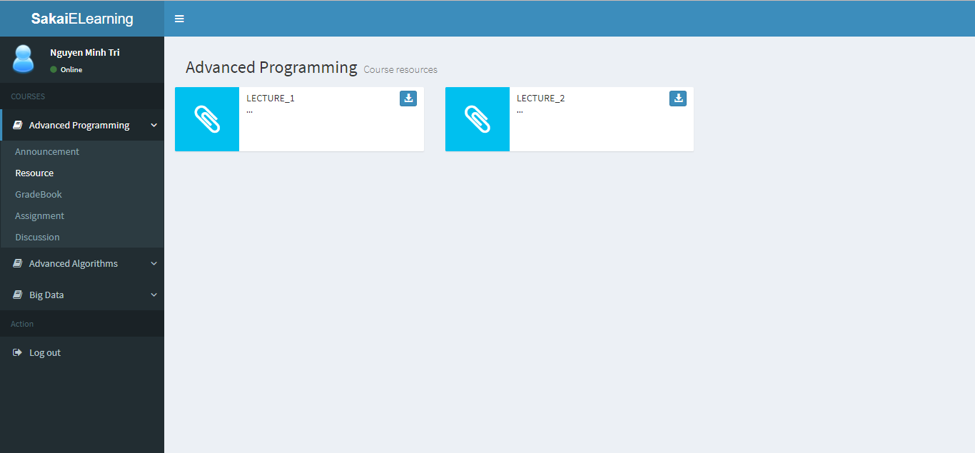
\includegraphics[scale = 1]{sakai6.png}
\caption{Trang chứa các tài nguyên của các môn học}
\end{figure}

\begin{figure}[H]
\centering
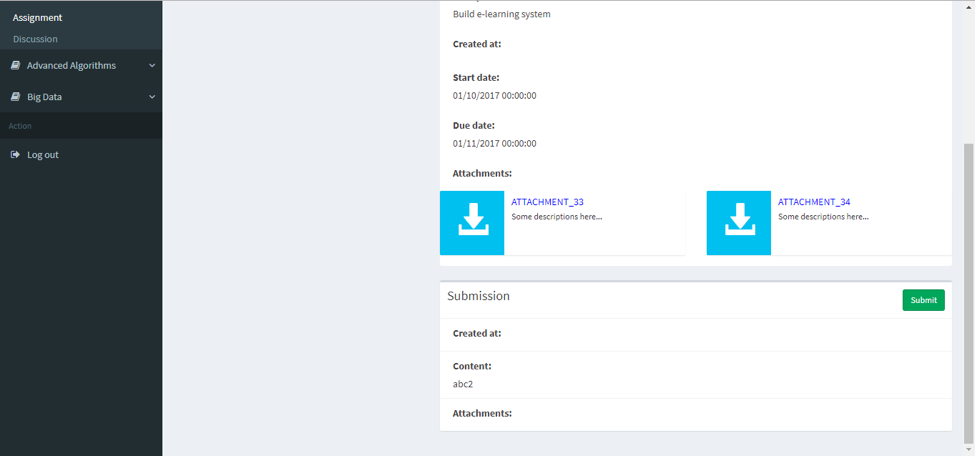
\includegraphics[scale = 1]{sakai7.png}
\caption{Trang nộp bài tập của sinh viên}
\end{figure}

%\bibliographystyle{plain}
%\bibliography{refs}
\section{Kết Luận}
Hệ thống đã đáp ứng được một số yêu cầu cơ bản của một hệ thống E-learning phục vụ học tập và giảng dạy cho khoa Khoa  và Kỹ Thuật Máy Tính. Hệ thống được xây dựng hoàn toàn bằng các thư viện mở do đó có khả năng phát triển tiếp trong tương lai với một số tính năng sau:
\begin{itemize}
\item Chức năng tự quản lý profile của người dùng.
\item Chức năng gửi mail thông báo.
\item Phát triển ứng dụng nhỏ trên điện thoại để nhận thông báo.
\end{itemize}

\end{document}